\section{Five Arms and the Decision Rule}
\label{sec:method}

\begin{figure}[t]
\centering
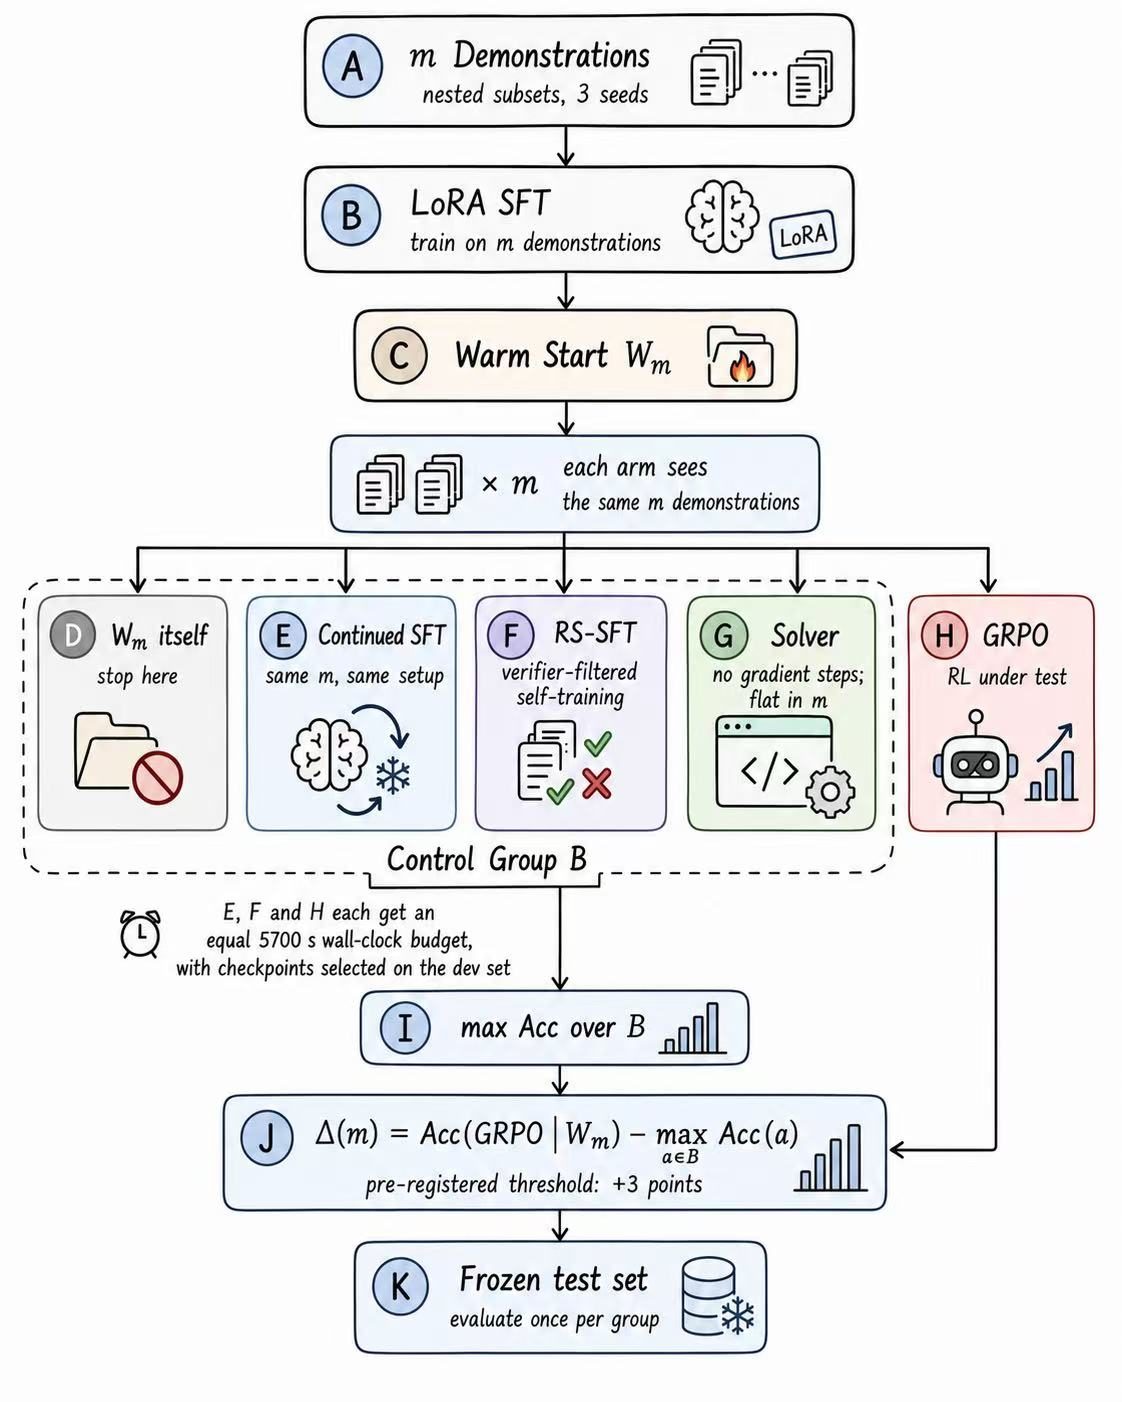
\includegraphics[width=0.92\textwidth]{figs/fig1_design.jpg}
\caption{The five arms and the decision rule. Every arm branches from the same
warm start $W_m$ and sees the same $m$ demonstrations, so the comparison is
about what to do next with a fixed budget. $\Delta$ takes the \emph{maximum}
over the four-arm control group $\mathcal{B}$.}
\label{fig:design}
\end{figure}

All arms branch from a common warm start $W_m$: a LoRA SFT run on the $m$
demonstrations of that budget and seed. This makes the comparison about
\emph{what to do next with the same $m$ demonstrations}, not about different
amounts of supervision.

\paragraph{The four baseline arms.}
$W_m$ itself is the starting point. \textbf{Continued SFT} keeps imitating the
same $m$ demonstrations under the same optimizer settings. \textbf{RS-SFT}
samples from the current policy on pool questions whose gold programs are
\emph{not} revealed, keeps verifier-accepted trajectories, and fine-tunes on
them, iterating. \textbf{The solver} is a deterministic program: it parses the
table, aligns question tokens to row and column labels through a cascade
(exact $\rightarrow$ normalized $\rightarrow$ fuzzy $\rightarrow$ year/numeric
$\rightarrow$ synonym), classifies the arithmetic intent, and emits a program.
Its \emph{scarce} variant---the protocol-compliant one---may retrieve from
exactly the $m$ gold programs of that budget, matching the demonstration
budget of the learning arms. A \emph{full} variant with access to the whole
pool is computed for diagnosis only and never enters $\mathcal{B}$.

\paragraph{The tested arm.}
GRPO~\cite{grpo2024} starts from the same $W_m$ and trains on pool questions
with the verifier as reward, under a wall-clock budget matched to continued SFT
and RS-SFT (Config~1: GRPO 5701--5728\,s, c-SFT 5703--5707\,s at $m{=}64$,
RS-SFT 4561--5815\,s). We note one budget asymmetry in the opposite direction
of our conclusion: at $m{=}2$ in Config~1, continued SFT converged in
2579--3196\,s against GRPO's 5701--5703\,s, so GRPO received more compute than
the baseline it is compared with.

\paragraph{Implementation and compute.}
All runs use PyTorch 2.10, \texttt{transformers} 4.57, \texttt{peft} 0.19 and
\texttt{trl} 1.8 on a single NVIDIA RTX A6000 (48\,GB) per run. All generation
uses HuggingFace \texttt{generate} throughout: we tested swapping in vLLM and
found it shifts accuracy by $3.00$ points---the same magnitude as our Go
threshold, and in no systematic direction---so the substitution was rejected
(Appendix~\ref{subsec:enginegate}). Every arm
trains a LoRA adapter ($r{=}16$, $\alpha{=}32$, dropout $0$) at learning rate
$10^{-5}$; GRPO uses 8 generations per prompt, KL coefficient $\beta{=}0.04$,
temperature $1.0$, top-$p$ $0.95$, and effective batch 64 (per-device 16,
accumulation 4), reduced to per-device 4 with accumulation 16 at 7B to fit the
card. Each arm is capped at 5700\,s of wall clock, enforced at step boundaries, so
runs may overshoot by one step. Checkpoints are selected on
dev; the test set is evaluated once per group. Section~\ref{sec:analysis}
reports the sweep over $\beta$, the only hyperparameter we
varied after the protocol was fixed.

\paragraph{Decision rule.}
$\Delta(m)$ follows Eq.~\eqref{eq:delta}. Comparison uses integer counts,
$k_{\text{GRPO}} - \max_a k_a \geq \lceil 0.03n \rceil$, to avoid
floating-point boundary effects at the $+3$-point Go threshold. Per-item
agreement is tested with McNemar and corrected with Holm.
Only ``GRPO vs.\ the strongest non-RL arm'' is confirmatory; everything else is
descriptive.

Where the threshold comes from matters for reading a null result, so we state it
rather than assert it. It was fixed between two anchors. The upper one is the
published literature. In the RLVR-for-finance papers we could compare against,
the gain from adding RL on top of SFT, measured on program-annotated financial
QA, runs from $-2.56$ to $+4.0$ points: Fin-R1 reports $+3.0$ on FinQA and
$+4.0$ on ConvFinQA~\cite{finr1_2025}, Fino1 $+1.25$ on
FinQA~\cite{fino1_2025}, and DianJin-R1 $-2.56$ on
FinQA~\cite{dianjinr1_2025}. A bar at five points would therefore have meant
``better than anything published on this task family.'' We restrict the
comparison to program-annotated QA deliberately and note what that excludes: the
one published figure we found that reaches five rather than falling below it is
Fin-R1's $+5.0$ on a benchmark that is not program synthesis. Within the task
family this paper studies, nothing published clears the bar. The lower anchor is
measurement resolution: we estimated single-seed
standard error at three to five points, which makes $+3$ the floor of what this
design can distinguish from seed noise at all. We set the Go criterion at the
lower anchor, $+3$, which is the more permissive of the two.

Because $+3$ therefore sits \emph{inside} the noise band of any single run, the
protocol never let it stand alone. A Go verdict additionally requires that at
least two of the three seeds in a cell be positive, that GRPO beat RS-SFT rather
than only plain SFT, and that the verifier-hacking audit be clean; and an effect
anywhere between two and five points, or one whose seeds disagree in sign, is
declared \textsc{inconclusive} and sent back for two further seeds rather than
adjudicated. The evidence this study rests on is accordingly agreement across
seeds and cells rather than per-group significance---which was the design, not a
retreat, as Section~\ref{sec:statistics} quantifies.

\paragraph{Solver cost.}
The solver is task-specific engineering, requiring roughly 440 new lines of
adaptation code on top of a reusable symbolic execution core. We report this
because the fair reading of our result is not ``a small script beats RL'' but
``a few hundred lines of task-specific symbolic code, which this benchmark
family admits by construction, beats RL under scarcity.''
